\documentclass{article}

\PassOptionsToPackage{numbers,compress}{natbib}
\usepackage[preprint]{neurips_2019}
\makeatletter
\renewcommand{\@noticestring}{}
\makeatother
\usepackage[utf8]{inputenc}
\usepackage[T1]{fontenc}
\usepackage{hyperref}
\usepackage{url}
\usepackage{xurl}
\usepackage{booktabs}
\usepackage{amsfonts}
\usepackage{amsmath}
\usepackage{microtype}
\usepackage{graphicx}
\graphicspath{{figures/}}

\title{Dreamer from Pixels: Additional Midterm Material}

\author{%
  Chevy Yang \\
  \texttt{chenyiy@andrew.cmu.edu}
  \And
  Zhiyuan Yang \\
  \texttt{dyang3@andrew.cmu.edu}
}

\begin{document}
\maketitle

\begin{center}
Team 25 \\
\textit{TA Mentor: Kangping Liu}
\end{center}

\begin{abstract}
This document provides additional evidence after the original midterm draft. We keep the completed 100k-environment-step Dreamer V1 baseline as the main reference, and add two separately labeled results: a longer seed-0 run that sampled 330,732 environment steps and a teammate-reported seed-1 run at 100,000 environment steps. The longer run evaluated a checkpoint representing 330,000 environment steps and obtained $322.0840 \pm 9.6868$ on ten evaluation episodes. Hao Deng's seed-1 summary reports $227.0931 \pm 29.4737$ under the 100k protocol. The seed-1 value is useful for discussion, but its raw configuration, per-episode CSV, and checkpoint were not available locally, so we do not treat it as independently verified evidence.
\end{abstract}

\section{Purpose and Scope}

Our project studies Dreamer V1 for visual control in the DeepMind Control Suite. We use the fixed PyTorch implementation by Julius Frost at commit \texttt{ccea6ae4a397a94c328891bd78e81d52dd156cb6}, with \texttt{rlpyt} at commit \texttt{f04f23db1eb7b5915d88401fca67869968a07a37}. The task is \texttt{cartpole\_swingup} with camera 0, 64 x 64 RGB observations, and action repeat 2. Dreamer learns a latent world model from image sequences and improves the actor and critic using imagined latent trajectories \citep{hafner2020dream}. The environment and reward contract come from the DeepMind Control Suite \citep{tassa2018dmcontrol}.

This addendum updates the empirical part of the midterm. It does not replace the earlier report's method description, proposal-aligned future work, or Chevy Yang's contribution description. It adds Zhiyuan Yang's longer seed-0 result and records the seed-1 result supplied by Hao Deng as a provisional team comparison.

\section{Protocol and Checkpoint Identity}

The formal 100k protocol uses 50,000 policy decisions, corresponding to 100,000 underlying environment steps. Episodes contain 500 decisions, or 1,000 environment steps. The replay capacity is 60,000 decision transitions; training uses batches of 16 sequences of length 50, a 1,000-decision prefill, updates every 1,000 decisions, and 100 optimizer updates per update cycle. The imagination horizon is 15. The run uses 32-bit precision and \texttt{use\_pcont=False}; no continuation-prediction loss is included in the world-model objective.

The longer seed-0 run used the same effective training configuration and stopped at its wall-clock limit. Its total interaction count was 165,366 decisions and 330,732 environment steps, with 16,500 optimizer updates. The reported final score belongs to \texttt{long\_train\_run/run\_0/params.pkl}, whose payload records \texttt{itr=164999}. Thus, the evaluated checkpoint represents 165,000 decisions, or 330,000 environment steps; the additional 732 environment steps are listed separately as total sampled interaction. This distinction matters because a checkpoint counter and the runner's final interaction count do not necessarily coincide at a non-boundary stop.

The formal initial policy is the same training model saved after prefill and before the first optimizer update. We do not create a separate random initialization to serve as the training-initial comparison. Each policy is evaluated on environment seeds 1000--1009 for ten episodes. Reported error bars are sample standard deviations across evaluation episodes, not variation across training seeds. Return is an episodic control metric, not a success rate.

\section{Additional Results}

Table~\ref{tab:additional} lists the three relevant final-policy results. The original seed-0 100k baseline is included as a reference point. The overnight seed-0 result is a different budget and is not concatenated with the 100k curve. Hao Deng's seed-1 result is reported at the same 100k budget as the reference baseline, but the raw files were not available locally for an independent audit.

\begin{table}[t]
\centering
\caption{Final Dreamer evaluation on ten episodes with environment seeds 1000--1009. The seed-1 row is a teammate-reported aggregate summary, not a locally reloaded checkpoint result.}
\label{tab:additional}
\small
\begin{tabular}{llllrr}
\toprule
Run & Training seed & Budget & Evidence & Mean & Sample std. \\
\midrule
Reference baseline & 0 & 100k env & local full artifact & 181.7011 & 27.5705 \\
Longer run & 0 & 330k checkpoint & local full artifact & 322.0840 & 9.6868 \\
Hao Deng run & 1 & 100k env & teammate summary & 227.0931 & 29.4737 \\
\bottomrule
\end{tabular}
\end{table}

\begin{figure}[t]
\centering
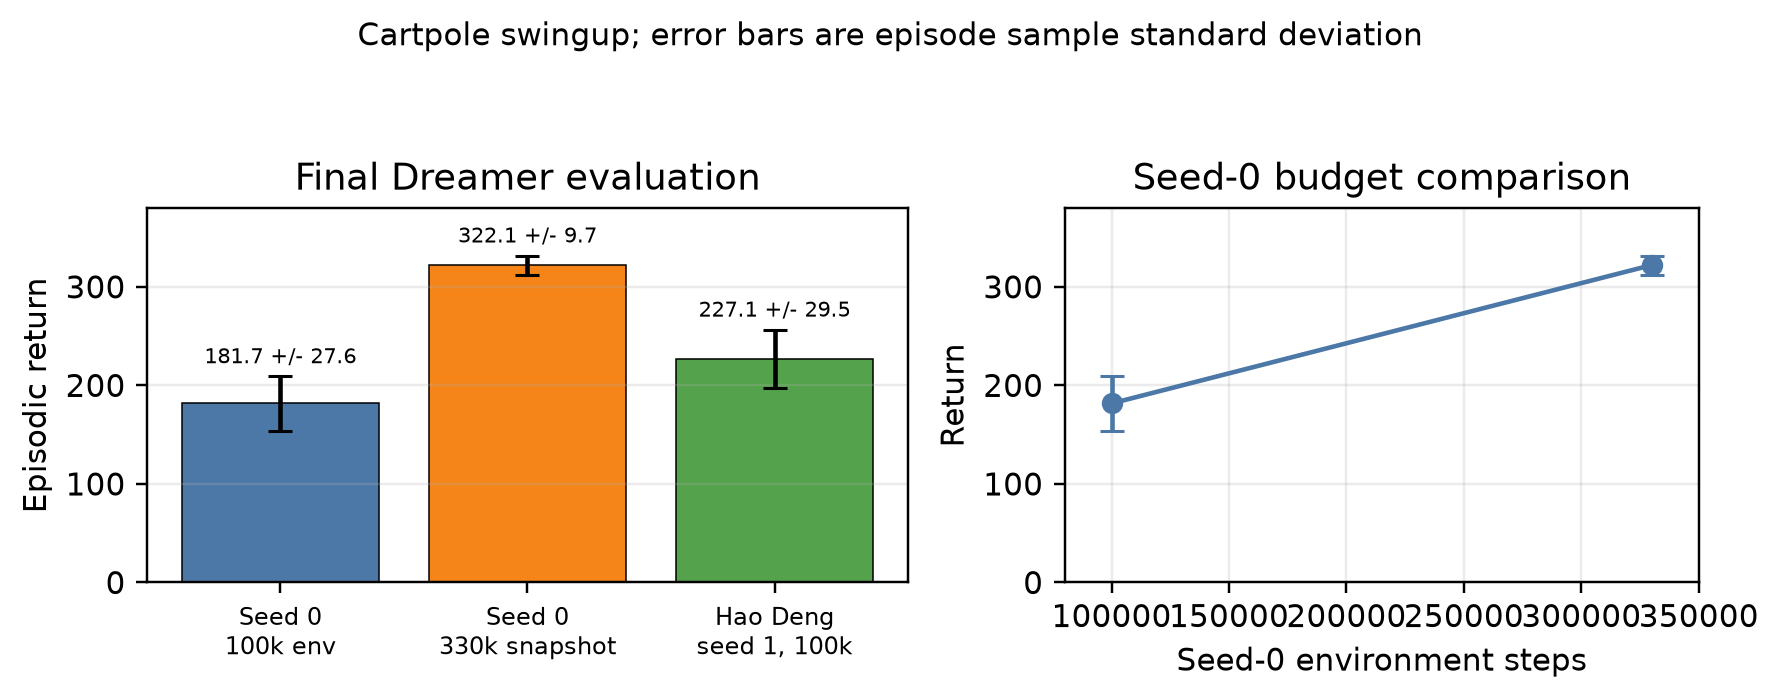
\includegraphics[width=0.98\linewidth]{additional_material_returns.png}
\caption{Additional comparison. Error bars are sample standard deviations over ten evaluation episodes. The seed-0 budget panel compares the independently evaluated 100k baseline with the longer run; it is not a learning curve. The seed-1 aggregate is shown without invented episode-level points because its raw CSV was not available locally.}
\label{fig:additional}
\end{figure}

The longer seed-0 policy scores higher than its own training-initial snapshot ($73.7413 \pm 2.3887$) and random control ($45.6311 \pm 37.4796$). Its mean return is still only about 322 out of the theoretical episodic maximum of 1,000. The increase over the original 100k seed-0 result is consistent with additional training, but the two runs also have different wall-clock histories and checkpointing, so this is not a controlled one-factor experiment. The final episodes are not evidence of statistical significance or stable mastery across training seeds.

Hao Deng's reported seed-1 result is above the reported seed-1 training-initial value ($71.9370 \pm 4.8223$) and random control ($45.1544 \pm 27.3207$). It is close enough in budget and headline protocol to motivate a cross-seed comparison, but the missing raw files limit what we can claim. In particular, we cannot independently verify the exact configuration, checkpoint identity, per-episode returns, or whether every source of evaluation randomness was controlled in the same way. We therefore do not compute a three-seed mean or standard deviation from this addendum.

\section{What This Evidence Supports}

The seed-0 overnight run supports a narrow engineering conclusion: the selected Dreamer V1 path can train substantially beyond 100k environment steps on the Kaggle GPU route, save a model, and produce a fresh-process evaluation. The observed return increase is an empirical result for one training seed and one task. It is not a reproduction of the paper's full benchmark suite.

The teammate result supports a weaker scientific conclusion: there is an additional 100k seed-1 report that can be compared provisionally with the 100k baseline. Because the evidence is aggregate-only, it should be treated as a lead for verification rather than a finalized multi-seed result. We should not pool the 20 reported evaluation episodes as if they were 20 training seeds, and we should not use the 330k seed-0 run as a second training seed.

\section{Limitations and Next Actions}

The most important missing item is Hao Deng's raw seed-1 package: the effective config, progress or training log, final and pre-update checkpoints, and per-episode evaluation CSV. Once supplied, we will compare the code commit, update schedule, replay capacity, step accounting, evaluation action rule, and environment-seed handling before publishing a matched cross-seed statistic. Until then, the table and figure preserve the provenance distinction.

Our next actions are concrete. First, verify the seed-1 raw artifacts and check the 100k protocol against the repository notebook. Second, keep the seed-0 330k result as a separate longer-budget experiment rather than mixing it into the 100k baseline. Third, after the baseline evidence is aligned, run the proposal's matched-budget experiments: imagination horizons such as 5, 15, and 30, and the proposed 4-pixel random-shift augmentation. Those extensions have not been executed here, and no improvement is assumed.

\section*{Team Contributions}

Chevy Yang's contribution description remains unchanged from the main report. Chevy and Zhiyuan Yang both contributed to the seed-0 Dreamer V1 baseline, including experiment setup, execution, and review of the resulting evidence. Zhiyuan Yang prepared the longer seed-0 run and this additional-material analysis. Hao Deng supplied the reported seed-1 training/evaluation summary; the detailed division of his implementation and experiment work should be confirmed against the raw files before the report is treated as final.

\section*{Repository and Sources}

The project repository is \url{https://github.com/DDaniel-code/dreamer-pixels}. The selected implementation is software rather than a paper citation \citep{frost_dreamer_pytorch}; the original Dreamer paper and the PlaNet predecessor provide the research context \citep{hafner2020dream,hafner2019latent}. All numerical claims in this addendum are labeled by evidence level and are based on the local overnight artifacts or the teammate-provided aggregate summary.

\begingroup
\footnotesize
\setlength{\bibsep}{0pt}
\bibliographystyle{plainnat}
\bibliography{dreamer_pixels_additional_material}
\endgroup

\end{document}
